\appendix
\chapter{Appendix}
\label{appendix}

\section{Rete Networks for the Queries of the Train Benchmark}

The Rete algorithm uses \emph{tuples} to represent the vertices (along with their properties), edges and subgraphs in the graph. The algorithm defines an asynchronous network of communicating nodes. The Rete networks has three layers:

\begin{itemize}
  \item The top level consists of \emph{input nodes} which are type-instance indexers for the model. Each input node indexes a certain vertex type or edge label. The actual graph element is indicated by a vertex/edge icon in the upper right corner of the Rete node.
  \item \emph{Worker nodes} perform a transformation on the output of their parent node(s) and propagate the results. Partial query results are represented in tuples and stored in the memory of the worker node thus allowing for incremental query reevaluation.
  \item The bottom level consist of \emph{production nodes} which are terminators that provide an interface for fetching the results of the query and the changes introduced by the latest transformation.
\end{itemize}

In \figref{fig:rete-poslength-layout}--\figref{fig:rete-signalneighbor-layout}, we present possible Rete networks layouts for the queries in the Train Benchmark.

\begin{figure}[htb]
\centering
\begin{minipage}[b]{0.4\textwidth}
\begin{center}
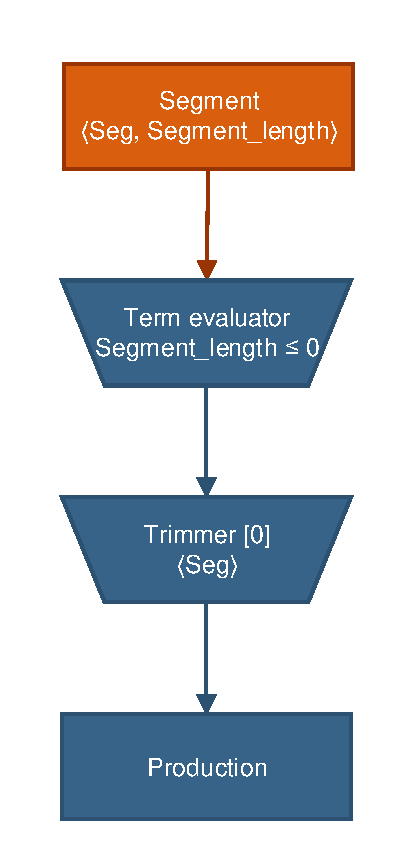
\includegraphics[scale=0.5]{figures/rete-poslength-layout.pdf}
\caption{The Rete network for the \textsf{PosLength} query.}
\label{fig:rete-poslength-layout}
\end{center}
\end{minipage}
\qquad
\begin{minipage}[b]{0.4\textwidth}
\begin{center}
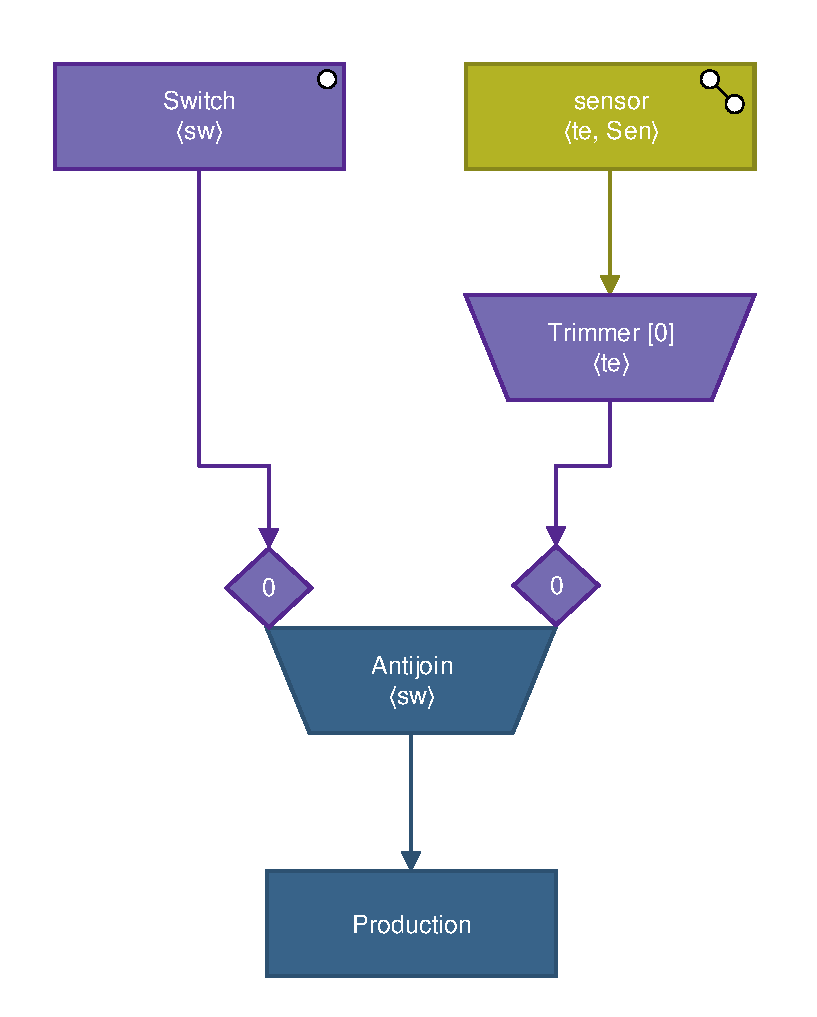
\includegraphics[scale=0.5]{figures/rete-switchsensor-layout.pdf}
\caption{The Rete network for the \textsf{SwitchSensor} query.}
\label{fig:rete-switchsensor-layout}
\end{center}
\end{minipage}
\end{figure}

%\begin{figure}[htb]
%\end{figure}

\begin{figure}[htb]
\begin{center}
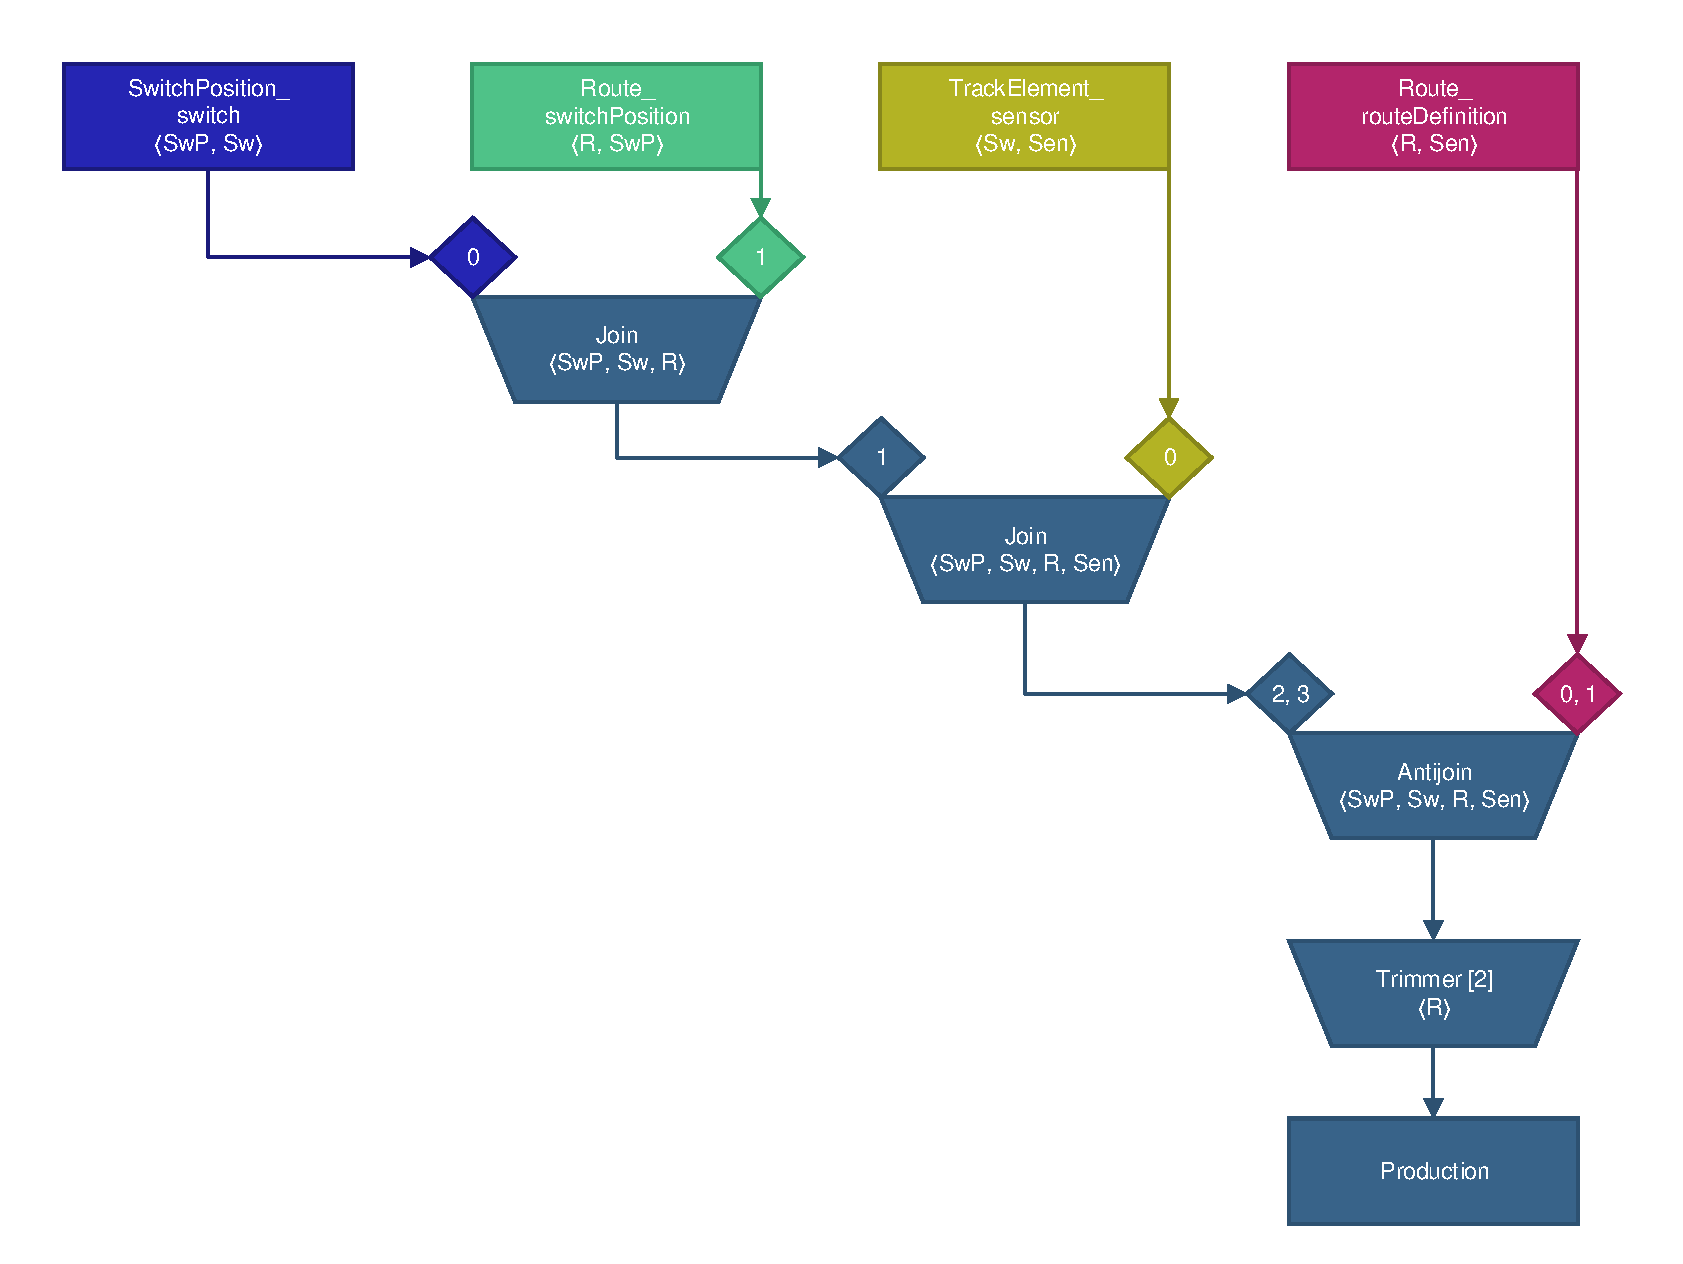
\includegraphics[scale=0.5]{figures/rete-routesensor-layout.pdf}
\caption{The Rete network for the \textsf{RouteSensor} query.}
\label{fig:rete-routesensor-layout}
\end{center}
\end{figure}

\begin{figure}[htb]
\begin{center}
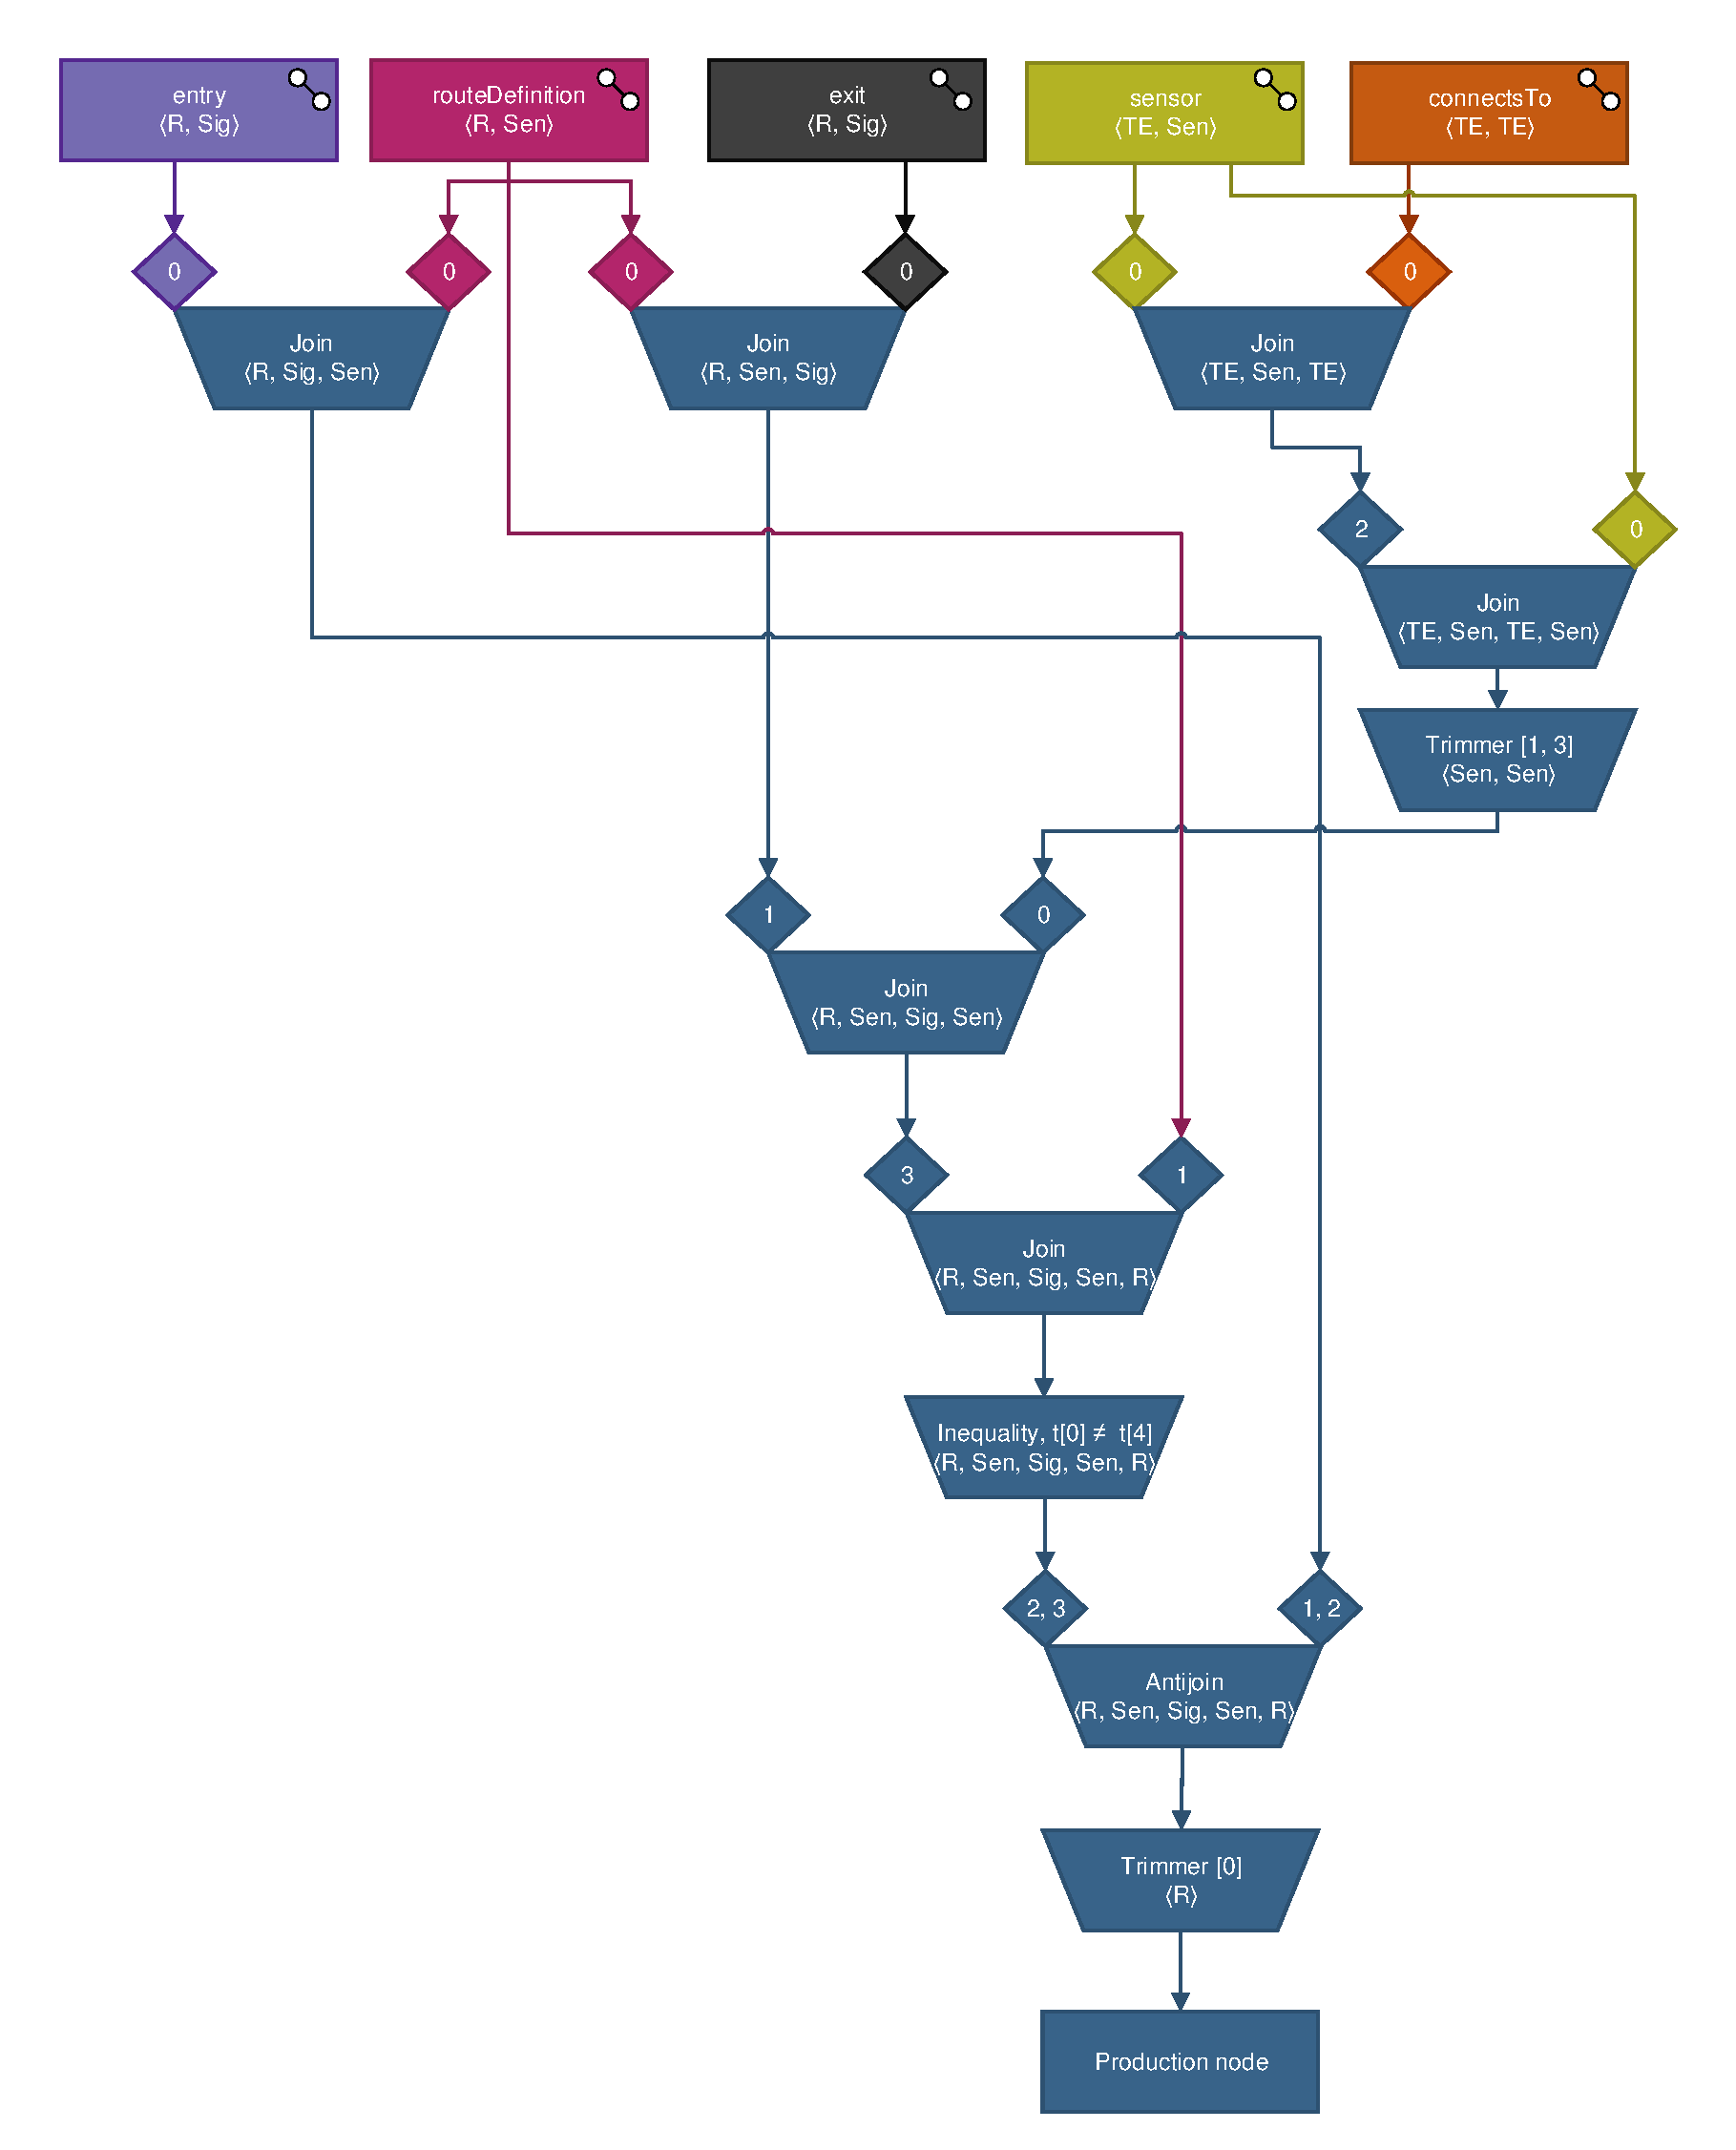
\includegraphics[scale=0.5]{figures/rete-signalneighbor-layout.pdf}
\caption{The Rete network for the \textsf{SignalNeighbor} query.}
\label{fig:rete-signalneighbor-layout}
\end{center}
\end{figure}
